%CHRIS: Antwort auf einen Delta-Impuls.
Die Gewichtsfunktion kann aus der Übertragungsfunktion durch Ableiten erhalten werden.
Alternativ kann die Gewichtsfunktion aus der Übertragungsfunktion durch Differention gewonnen werden.
%Die Lösung von Matlab ist zwar die gleiche, aber in einer anderen Darstellung. Sollte Matlab einen zu langen Ausdruck ausgeben, kann der Befehl simplify(ans) verwendet werden, um den Ausdruck zu vereinfachen.
...
\subsection{Parametrische Darstellung} %NICHT SICHER
Die Parametrische Darstellung der Gewichtsfunktion $g(t)$ erhält man, indem man die Laplace-Rücktransformierte der Übertragungsfunktion bildet. Das macht man wie folgt: 
%syms s -> G(s)=bspw. 3*s/(1+9*s + 20*s^2) -> ilaplace(G(s)) -> t=[0;0.1;10] -> plot(t, Antwort der parametrischen Darstellung) (Da t ein Vektor ist, muss man beim Multiplizieren das Punktprodukt (Hadamad-Produkt) .* verwenden) (Alternativ kann man das mit dem fplot befehl machen, da spart man sich das Hadamad-Produkt) -> xlabel (Mit den Befehlen xlabel und ylabel kann man die Achsen beschriften) -> ylabel Gewichtsfunktion
%texttt{sys=tf([..][..])}
%texttt{syms s \\ ...}
Das macht man wie folgt:
\texttt{syms s}\\
\texttt{syms t}\\
\texttt{G(s)=-25/(10*s+1)}\\
\texttt{g(t)=ilaplace(G(s))}\\
Matlab liefert hier $g(t)=-\frac{5*e^{\frac{-t}{10}}}{2}$
\subsection{Nichtparametrische Darstellung}
\subsubsection{Plot mit Matlab}
Mit der parametrischen Darstellung kann die Gewichtsfunktion in Matlab geplottet werden.
Hier graphisch dargestellt:\\
\texttt{t=[0:0.1:50]}\\
\texttt{t,-(5*exp(-t/10))/2}

\begin{figure}[H]
    \centering
    \includegraphics[width=5cm]{image/ImpulsantwortPlotinMatlab.eps}
    \caption{Impulsantwort: Plot in Matlab}
\end{figure}


\subsubsection{Plot mit Step-Funktion}
Den selben Plot bekommt man auch über die Matlab \texttt{impulse} Funktion\\
\texttt{sys=tf([-25], [10 1])}
\texttt{impulse(sys)}
\begin{figure}[H]
    \centering
    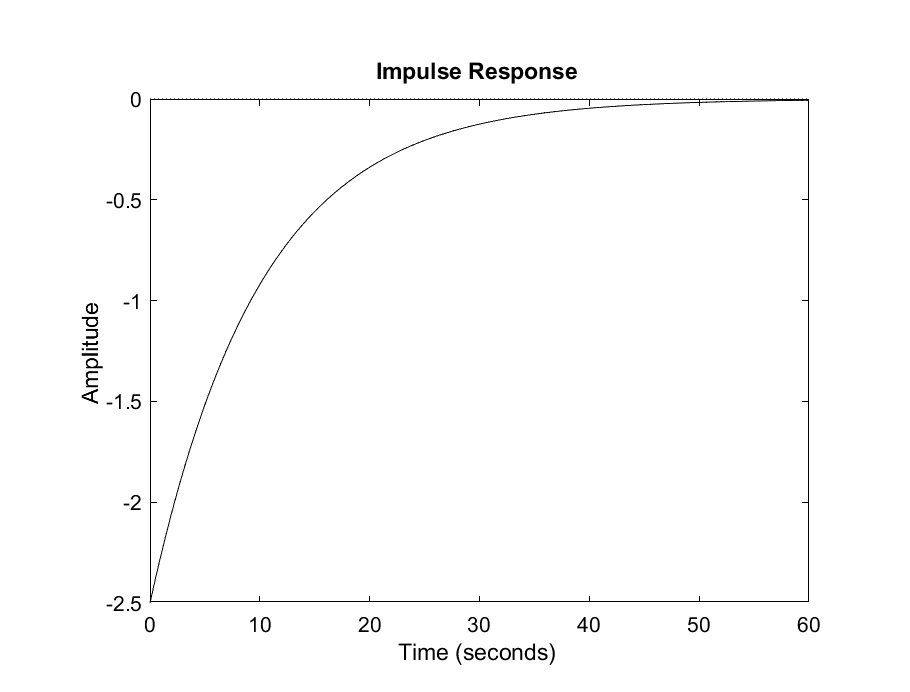
\includegraphics[width=5cm]{image/ImpulsantwortPlotmitImpulsFunktion.eps}
    \caption{Impulsantwort: Plot mit Impuls Funktion}
\end{figure}

\subsubsection{Plot mit Simulink}
...